% Provenance (never printed): cycle 3 "La planete Terre. Les etres vivants
% dans leur environnement" (natural phenomena: volcanoes and earthquakes,
% natural hazards and the behaviour to adopt); see sources/book1/PROVENANCE.md.
% Book 1, grade 4, chapter 2.
\chapter{Volcanoes and Earthquakes: A First Look}\label{ch:g4:volcanoes-earthquakes-first-look}

On Monday evening, the news shows a \omterm{def:g4:volcanoes-earthquakes-first-look:volcano}{volcano} on an island far away. In the
dark, a fountain of glowing orange \omterm{def:g3:stones-pebbles-sand:rock}{rock} spurts from a crack in the ground,
and \omterm{def:g1:landscapes-around-us:water}{rivers} of fire flow slowly down the slope into the \omterm{def:g2:water-on-earth:ocean}{sea}, hissing and
steaming. On Thursday, the news shows another place: a small town where,
at dawn, the ground shook for half a minute. Chimneys fell into the street,
and one old house slid off its base.

Two very different events. Yet both come from deep inside the Earth, and,
as we shall see, both happen far more often in some parts of the world than
in others.

\begin{recall}
\omterm{def:g1:landscapes-around-us:landform}{Mountains}, \omterm{def:g1:landscapes-around-us:landform}{hills}, \omterm{def:g1:landscapes-around-us:landform}{valleys} and \omterm{def:g1:landscapes-around-us:landform}{plains} are the shapes of the land
(\cref{ch:g1:landscapes-around-us}). The Earth's land is gathered in seven
\omterm{def:g3:continents-and-oceans:continent}{continents}, between five \omterm{def:g2:water-on-earth:ocean}{oceans}; the Pacific is the largest \omterm{def:g2:water-on-earth:ocean}{ocean}
(\cref{ch:g3:continents-and-oceans}).
\end{recall}

\section{A volcano erupts}

Deep under our feet, the Earth is very hot. In some places, \omterm{def:g3:stones-pebbles-sand:rock}{rock} down there
is so hot that it has melted. This molten \omterm{def:g3:stones-pebbles-sand:rock}{rock} is lighter than the solid
\omterm{def:g3:stones-pebbles-sand:rock}{rock} around it, so it slowly rises, like a cork in water. Where it finds a
way out to the surface, a \omterm{def:g4:volcanoes-earthquakes-first-look:volcano}{volcano} is born.

\begin{definition}[Volcano]\label{def:g4:volcanoes-earthquakes-first-look:volcano}
A \emph{volcano}\index{volcano} is a place where molten \omterm{def:g3:stones-pebbles-sand:rock}{rock} from deep
inside the Earth comes out at the surface, and the \omterm{def:g1:landscapes-around-us:landform}{hill} or \omterm{def:g1:landscapes-around-us:landform}{mountain} that
the molten \omterm{def:g3:stones-pebbles-sand:rock}{rock} builds there, layer after layer.
\end{definition}

\begin{definition}[Eruption, lava and volcanic ash]\label{def:g4:volcanoes-earthquakes-first-look:eruption}
An \emph{eruption}\index{eruption} is the time when a \omterm{def:g4:volcanoes-earthquakes-first-look:volcano}{volcano} throws out
molten \omterm{def:g3:stones-pebbles-sand:rock}{rock}, ash and gas. \emph{Lava}\index{lava} is molten \omterm{def:g3:stones-pebbles-sand:rock}{rock} that
pours out onto the surface; it flows, then cools and hardens into new \omterm{def:g3:stones-pebbles-sand:rock}{rock}.
\emph{Volcanic ash}\index{volcanic ash} is made of tiny pieces of \omterm{def:g3:stones-pebbles-sand:rock}{rock} and
glass blown into the air by an eruption; it falls back like a grey \omterm{def:g4:clouds-rain-snow:precipitation}{snow}.
\end{definition}

\begin{omfigure}
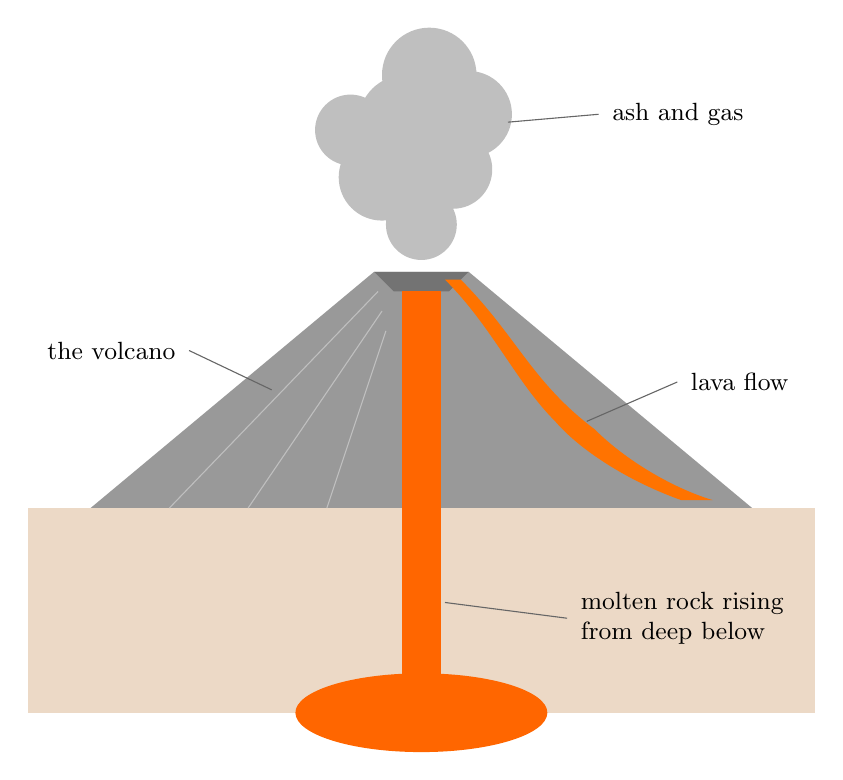
\begin{tikzpicture}[font=\small]
  % ground and deep rock
  \fill[brown!30] (-5,-2.6) rectangle (5,0);
  % the volcano
  \fill[black!40] (-4.2,0) -- (-0.6,3.0) -- (0.6,3.0) -- (4.2,0) -- cycle;
  \fill[black!55] (-0.6,3.0) -- (-0.35,2.75) -- (0.35,2.75) -- (0.6,3.0) -- cycle;
  % layers inside the cone
  \foreach \k in {1,2,3}
    \draw[black!25] (-4.2+1.0*\k,0) -- (-0.6+0.05*\k,3.0-0.25*\k);
  % molten rock rising from deep below
  \fill[orange!80!red] (-0.25,-2.6) -- (-0.25,2.75) -- (0.25,2.75) -- (0.25,-2.6) -- cycle;
  \fill[orange!80!red] (0,-2.6) ellipse (1.6 and 0.5);
  % lava flow on the right flank
  \fill[orange!90!red] (0.5,2.9) .. controls (1.2,2.2) and (1.4,1.6) .. (2.2,1.0)
    .. controls (2.6,0.6) and (3.2,0.25) .. (3.7,0.1) -- (3.3,0.1)
    .. controls (2.6,0.35) and (2.0,0.75) .. (1.7,1.1)
    .. controls (1.2,1.6) and (0.9,2.3) .. (0.3,2.9) -- cycle;
  % ash and gas cloud
  \foreach \x/\y/\r in {0/3.6/0.45, -0.5/4.2/0.55, 0.4/4.3/0.5, -0.2/4.9/0.6, 0.6/5.0/0.55, -0.9/4.8/0.45, 0.1/5.5/0.6}
    \fill[black!25] (\x,\y) circle (\r);
  % labels
  \node[anchor=west] at (2.3,5.0) {ash and gas};
  \draw[black!60] (2.25,5.0) -- (1.1,4.9);
  \node[anchor=west] at (3.3,1.6) {lava flow};
  \draw[black!60] (3.25,1.6) -- (2.1,1.1);
  \node[anchor=east] at (-3.0,2.0) {the volcano};
  \draw[black!60] (-2.95,2.0) -- (-1.9,1.5);
  \node[anchor=west, align=left] at (1.9,-1.4) {molten rock rising\\from deep below};
  \draw[black!60] (1.85,-1.4) -- (0.3,-1.2);
\end{tikzpicture}

{\small A \omterm{def:g4:volcanoes-earthquakes-first-look:volcano}{volcano} erupting (drawn, not to scale). Molten \omterm{def:g3:stones-pebbles-sand:rock}{rock} rises from
deep below and comes out at the top: it flows down as \omterm{def:g4:volcanoes-earthquakes-first-look:eruption}{lava}, while ash and
gas are blown up into the sky. Each \omterm{def:g4:volcanoes-earthquakes-first-look:eruption}{eruption} adds a new layer to the
\omterm{def:g1:landscapes-around-us:landform}{mountain}.}
\label{fig:g4:volcanoes-earthquakes-first-look:volcano}
\end{omfigure}

Not all \omterm{def:g4:volcanoes-earthquakes-first-look:eruption}{eruptions} look alike. In some, the \omterm{def:g4:volcanoes-earthquakes-first-look:eruption}{lava} is runny: it pours out
quietly in glowing \omterm{def:g1:landscapes-around-us:water}{rivers} that can flow for kilometres, sometimes all the
way to the \omterm{def:g2:water-on-earth:ocean}{sea}. In others, the molten \omterm{def:g3:stones-pebbles-sand:rock}{rock} is thick and full of gas, like
a shaken bottle of fizzy drink: when it bursts out, it explodes into a huge
column of ash that rises high into the sky.

\begin{omfigure}
\begin{minipage}[b]{0.56\linewidth}\centering
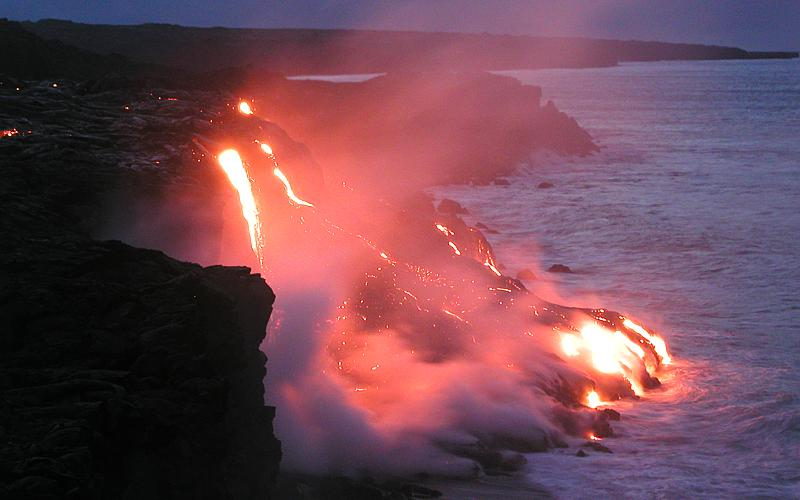
\includegraphics[width=\linewidth]{images/book1/g4-lava-ocean.jpg}

{\small A runny \omterm{def:g4:volcanoes-earthquakes-first-look:eruption}{eruption}: \omterm{def:g4:volcanoes-earthquakes-first-look:eruption}{lava} pours down a \omterm{def:g2:water-on-earth:ocean}{sea} cliff into the \omterm{def:g2:water-on-earth:ocean}{ocean}, in
Hawaii. Photograph: USGS Hawaiian Volcano Observatory (public domain).}
\end{minipage}\hfill
\begin{minipage}[b]{0.4\linewidth}\centering
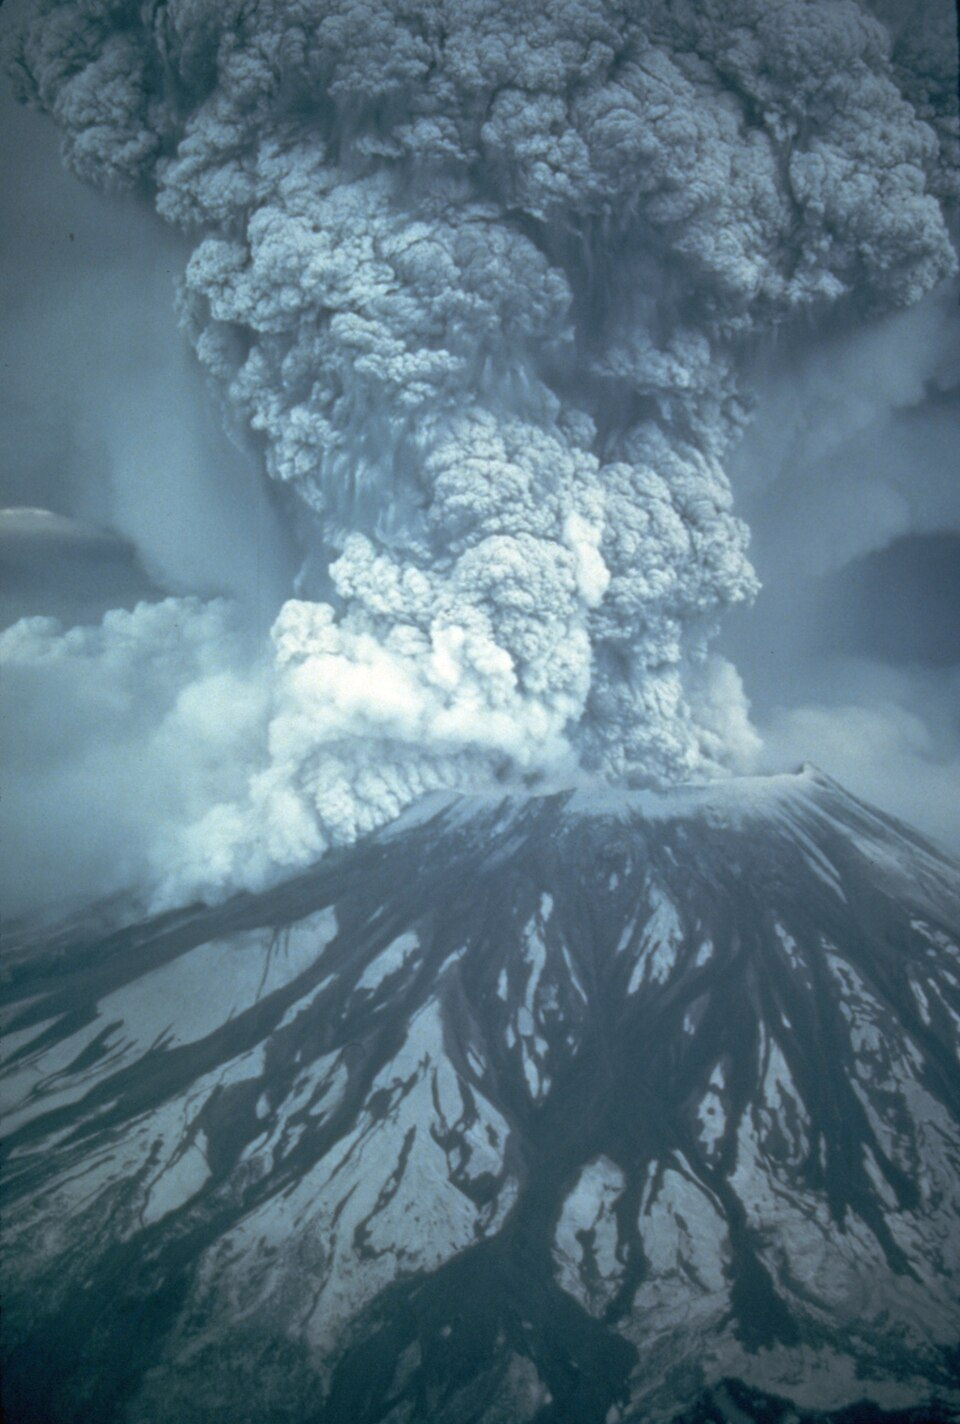
\includegraphics[width=0.78\linewidth]{images/book1/g4-st-helens.jpg}

{\small An explosive \omterm{def:g4:volcanoes-earthquakes-first-look:eruption}{eruption}: Mount St.~Helens, United States, 18~May
1980. Photograph: Austin Post, USGS (public domain).}
\end{minipage}
% ledger: usgs:pu-oo-ocean, usgs:msh-1980
\label{fig:g4:volcanoes-earthquakes-first-look:two-eruptions}
\end{omfigure}

\begin{example}[Mount St.~Helens, 1980]\label{ex:g4:volcanoes-earthquakes-first-look:st-helens}
In the spring of 1980, a bulge grew on the side of Mount
St.~Helens, as molten \omterm{def:g3:stones-pebbles-sand:rock}{rock} pushed up inside the \omterm{def:g1:landscapes-around-us:landform}{mountain}. On the morning
of 18~May, a small \omterm{def:g4:volcanoes-earthquakes-first-look:earthquake}{earthquake} shook the \omterm{def:g1:landscapes-around-us:landform}{mountain}, the bulge slid away in a
giant landslide, and the \omterm{def:g4:volcanoes-earthquakes-first-look:volcano}{volcano} exploded sideways and upwards. The top
400~metres of the \omterm{def:g1:landscapes-around-us:landform}{mountain} were gone: the summit became a huge crater.
% ledger: usgs:msh-1980
\end{example}

\section{The ground shakes}

The \omterm{def:g3:stones-pebbles-sand:rock}{rocks} deep under our feet are not perfectly still. Very slowly, they
are pushed and pulled. They bend a little, like a ruler you push at both
ends --- until, suddenly, they break and slip. The jolt sends the ground
shaking for kilometres all around.

\begin{definition}[Earthquake]\label{def:g4:volcanoes-earthquakes-first-look:earthquake}
An \emph{earthquake}\index{earthquake} is a sudden shaking of the ground,
caused by \omterm{def:g3:stones-pebbles-sand:rock}{rocks} that break and slip, deep underground.
\end{definition}

An \omterm{def:g4:volcanoes-earthquakes-first-look:earthquake}{earthquake} usually lasts only a few seconds, sometimes a minute or two
for the largest. Most \omterm{def:g4:volcanoes-earthquakes-first-look:earthquake}{earthquakes} are so small that nobody feels them: only
instruments notice them. A strong one can make the ground roll like the
deck of a ship, crack roads, and bring down walls and houses.

\begin{omfigure}
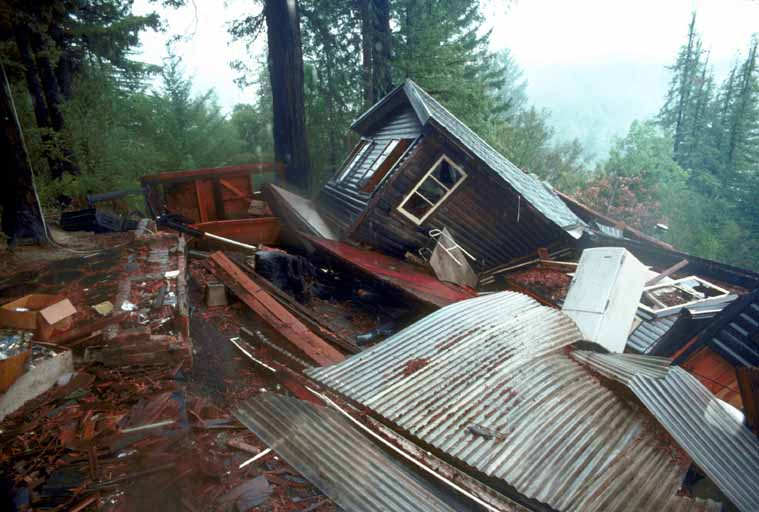
\includegraphics[width=0.55\linewidth]{images/book1/g4-loma-prieta-house.jpg}

{\small After a strong \omterm{def:g4:volcanoes-earthquakes-first-look:earthquake}{earthquake} in California in 1989: this wooden house
was thrown sideways off its concrete base. Photograph: J.~K.~Nakata, USGS
(public domain).}
% ledger: usgs:loma-prieta-house
\end{omfigure}

\begin{remark}[How often?]\label{rem:g4:volcanoes-earthquakes-first-look:how-often}
Geologists keep a list of all the large \omterm{def:g4:volcanoes-earthquakes-first-look:earthquake}{earthquakes} on Earth. Over the 50
years from 1976 to 2025, the list counts 7\,031 large ones (strong enough to
damage buildings near them): about 141 in a year, or almost 3 every week.
The very largest, which can destroy whole towns, are about 14 in a year.
Over the same Earth, about 1\,200 \omterm{def:g4:volcanoes-earthquakes-first-look:volcano}{volcanoes} have erupted in the last
twelve thousand years or so.
% ledger: data:usgs-comcat, data:gvp
\end{remark}

\section{Where volcanoes and earthquakes happen}

If \omterm{def:g4:volcanoes-earthquakes-first-look:volcano}{volcanoes} and \omterm{def:g4:volcanoes-earthquakes-first-look:earthquake}{earthquakes} happened anywhere at random, the dots on a
\omterm{def:g3:continents-and-oceans:world-map}{world map} would be sprinkled evenly over it. They are not.

The \omterm{def:g2:drawing-to-map:map}{map} below shows a striking pattern. Most \omterm{def:g4:volcanoes-earthquakes-first-look:volcano}{volcanoes} and most large
\omterm{def:g4:volcanoes-earthquakes-first-look:earthquake}{earthquakes} lie in long, narrow belts. The longest of all runs round the
Pacific \omterm{def:g2:water-on-earth:ocean}{Ocean}: from New Zealand up through Indonesia, the Philippines and
Japan, across to Alaska, then all the way down the west \omterm{def:g1:landscapes-around-us:water}{coast} of the
Americas to the tip of Chile. Because of its many \omterm{def:g4:volcanoes-earthquakes-first-look:volcano}{volcanoes}, it is often
called the ``Ring of Fire''.

\begin{example}[Counting on the map]\label{ex:g4:volcanoes-earthquakes-first-look:shares}
We counted the dots that lie in the shaded ring (within 500~kilometres of
its middle line). Of the 1\,214 \omterm{def:g4:volcanoes-earthquakes-first-look:volcano}{volcanoes}, 837 are in the ring: about 2 out
of every 3. Of the 696 very large \omterm{def:g4:volcanoes-earthquakes-first-look:earthquake}{earthquakes}, 532 are in the ring: about
3 out of every 4. The ring covers only a small part of the Earth, but it
holds most of its \omterm{def:g4:volcanoes-earthquakes-first-look:volcano}{volcanoes} and \omterm{def:g4:volcanoes-earthquakes-first-look:earthquake}{earthquakes}.
% ledger: data:gvp, data:usgs-comcat
\end{example}

\begin{omfigure}
\begin{tikzpicture}
\begin{axis}[ommap, width=\linewidth, xtick=\empty, ytick=\empty, grid=none,
    legend style={font=\scriptsize, at={(0.5,-0.02)}, anchor=north,
      draw=none, legend columns=3, /tikz/every even column/.append style={column sep=6pt}},
    legend cell align=left]
  \addplot[fill=omHypsLandA!85!black, draw=black!45, line width=0.2pt, forget plot]
    table {figdata/out/shared-geo-land.dat};
  \addplot[orange!80!black, opacity=0.35, line width=9pt, line cap=round, line join=round]
    table {figdata/out/grade-4-ring_of_fire-ring.dat};
  \addlegendentry{the ring around the Pacific}
  \addplot[only marks, mark=triangle*, mark size=1.3pt, red!75!black]
    table[x=lon, y=lat] {figdata/out/grade-4-ring_of_fire-volcanoes.dat};
  \addlegendentry{a volcano (last 12\,000 years)}
  \addplot[only marks, mark=*, mark size=1.0pt, black, fill opacity=0.6]
    table[x=lon, y=lat] {figdata/out/grade-4-ring_of_fire-quakes7.dat};
  \addlegendentry{a very large earthquake (1976--2025)}
\end{axis}
\end{tikzpicture}

{\small \omterm{def:g4:volcanoes-earthquakes-first-look:volcano}{Volcanoes} that have erupted in the last twelve thousand years or
so, and the very largest \omterm{def:g4:volcanoes-earthquakes-first-look:earthquake}{earthquakes} of 1976--2025. Most of them lie along
a ring of island chains and \omterm{def:g1:landscapes-around-us:landform}{mountain} ranges around the Pacific \omterm{def:g2:water-on-earth:ocean}{Ocean}
(shaded). Data: Smithsonian Global Volcanism Program; U.S. Geological
Survey \omterm{def:g4:volcanoes-earthquakes-first-look:earthquake}{earthquake} catalogue; coastlines Natural Earth.}
\label{fig:g4:volcanoes-earthquakes-first-look:map}
% ledger: data:gvp, data:usgs-comcat, data:ne-land
\end{omfigure}

Other belts are smaller: one crosses southern Europe and Asia, from the
Mediterranean \omterm{def:g2:water-on-earth:ocean}{Sea} to the Himalaya; others run down the middle of the
\omterm{def:g2:water-on-earth:ocean}{oceans}, where \omterm{def:g4:volcanoes-earthquakes-first-look:volcano}{volcanoes} are hidden under the water. Some places, like
Hawaii, have \omterm{def:g4:volcanoes-earthquakes-first-look:volcano}{volcanoes} far from any belt. Why the belts are where they are
is a question for \cref{ch:g7:plate-tectonics}: the answer explains the shape of the whole \omterm{def:g2:drawing-to-map:map}{map}.

\section{Staying safe}

Nobody can stop an \omterm{def:g4:volcanoes-earthquakes-first-look:eruption}{eruption} or an \omterm{def:g4:volcanoes-earthquakes-first-look:earthquake}{earthquake}. But knowing what to do saves
lives.

\begin{omfigure}
\begin{tikzpicture}[font=\small, line cap=round, line join=round]
  % --- panel 1: DROP onto hands and knees
  \begin{scope}
    \draw[black!30] (-0.2,0) -- (2.8,0);
    \fill[omDef] (0.62,0.98) circle (0.21);
    \draw[omDef, line width=2.2pt] (0.88,0.98) -- (2.0,0.95);
    \draw[omDef, line width=2pt] (0.95,0.96) -- (0.95,0.05);
    \draw[omDef, line width=2pt] (2.0,0.95) -- (1.98,0.08) -- (2.65,0.08);
    \node[font=\bfseries] at (1.3,-0.45) {DROP};
    \node[font=\scriptsize, align=center] at (1.3,-0.95) {onto your hands\\and knees};
  \end{scope}
  % --- panel 2: COVER under a table
  \begin{scope}[xshift=4cm]
    \draw[black!30] (-0.2,0) -- (2.8,0);
    \fill[brown!60!black] (-0.1,1.45) rectangle (2.7,1.6);
    \draw[brown!60!black, line width=2pt] (0.1,1.45) -- (0.1,0) (2.5,1.45) -- (2.5,0);
    \fill[omDef] (0.75,0.95) circle (0.2);
    \draw[omDef, line width=2.2pt] (0.95,0.85) -- (1.95,0.8);
    \draw[omDef, line width=2pt] (1.9,0.8) -- (1.65,0.05) -- (2.25,0.05);
    \draw[omDef, line width=2pt] (1.0,0.85) -- (0.7,1.2) -- (0.5,0.95);
    \node[font=\bfseries] at (1.3,-0.45) {COVER};
    \node[font=\scriptsize, align=center] at (1.3,-0.95) {your head and neck,\\under a sturdy table};
  \end{scope}
  % --- panel 3: HOLD ON to the table leg
  \begin{scope}[xshift=8cm]
    \draw[black!30] (-0.2,0) -- (2.8,0);
    \fill[brown!60!black] (-0.1,1.45) rectangle (2.7,1.6);
    \draw[brown!60!black, line width=2pt] (0.1,1.45) -- (0.1,0) (2.5,1.45) -- (2.5,0);
    \fill[omDef] (0.75,0.95) circle (0.2);
    \draw[omDef, line width=2.2pt] (0.95,0.85) -- (1.95,0.8);
    \draw[omDef, line width=2pt] (1.9,0.8) -- (1.65,0.05) -- (2.25,0.05);
    \draw[omDef, line width=2pt] (1.0,0.85) -- (0.7,1.2) -- (0.5,0.95);
    \draw[omDef, line width=2pt] (1.0,0.8) -- (0.45,0.6) -- (0.12,0.65);
    \node[font=\bfseries] at (1.3,-0.45) {HOLD ON};
    \node[font=\scriptsize, align=center] at (1.3,-0.95) {to the table until\\the shaking stops};
  \end{scope}
\end{tikzpicture}

{\small What to do as soon as the ground starts to shake: drop, cover and
hold on.}
\label{fig:g4:volcanoes-earthquakes-first-look:drop-cover}
% ledger: shakeout:dch
\end{omfigure}

\begin{safety}
\textbf{In an \omterm{def:g4:volcanoes-earthquakes-first-look:earthquake}{earthquake}.} As soon as you feel the ground shake:
\textbf{drop} onto your hands and knees; \textbf{cover} your head and neck
with your arm, and crawl under a sturdy table or desk if one is near;
\textbf{hold on} to it until the shaking stops. Do not run outside while
the ground shakes, and do not stand in a doorway: falling glass and objects
are the main danger. When it stops, leave the building calmly, as you
practise in school drills.

\textbf{Near a \omterm{def:g4:volcanoes-earthquakes-first-look:volcano}{volcano}.} Scientists watch \omterm{def:g4:volcanoes-earthquakes-first-look:volcano}{volcanoes} that may wake up. If
they warn that an \omterm{def:g4:volcanoes-earthquakes-first-look:eruption}{eruption} is coming, the authorities tell people to leave
the area. Follow their instructions at once, and never go closer to watch.
\end{safety}
% ledger: shakeout:dch

\begin{omfigure}
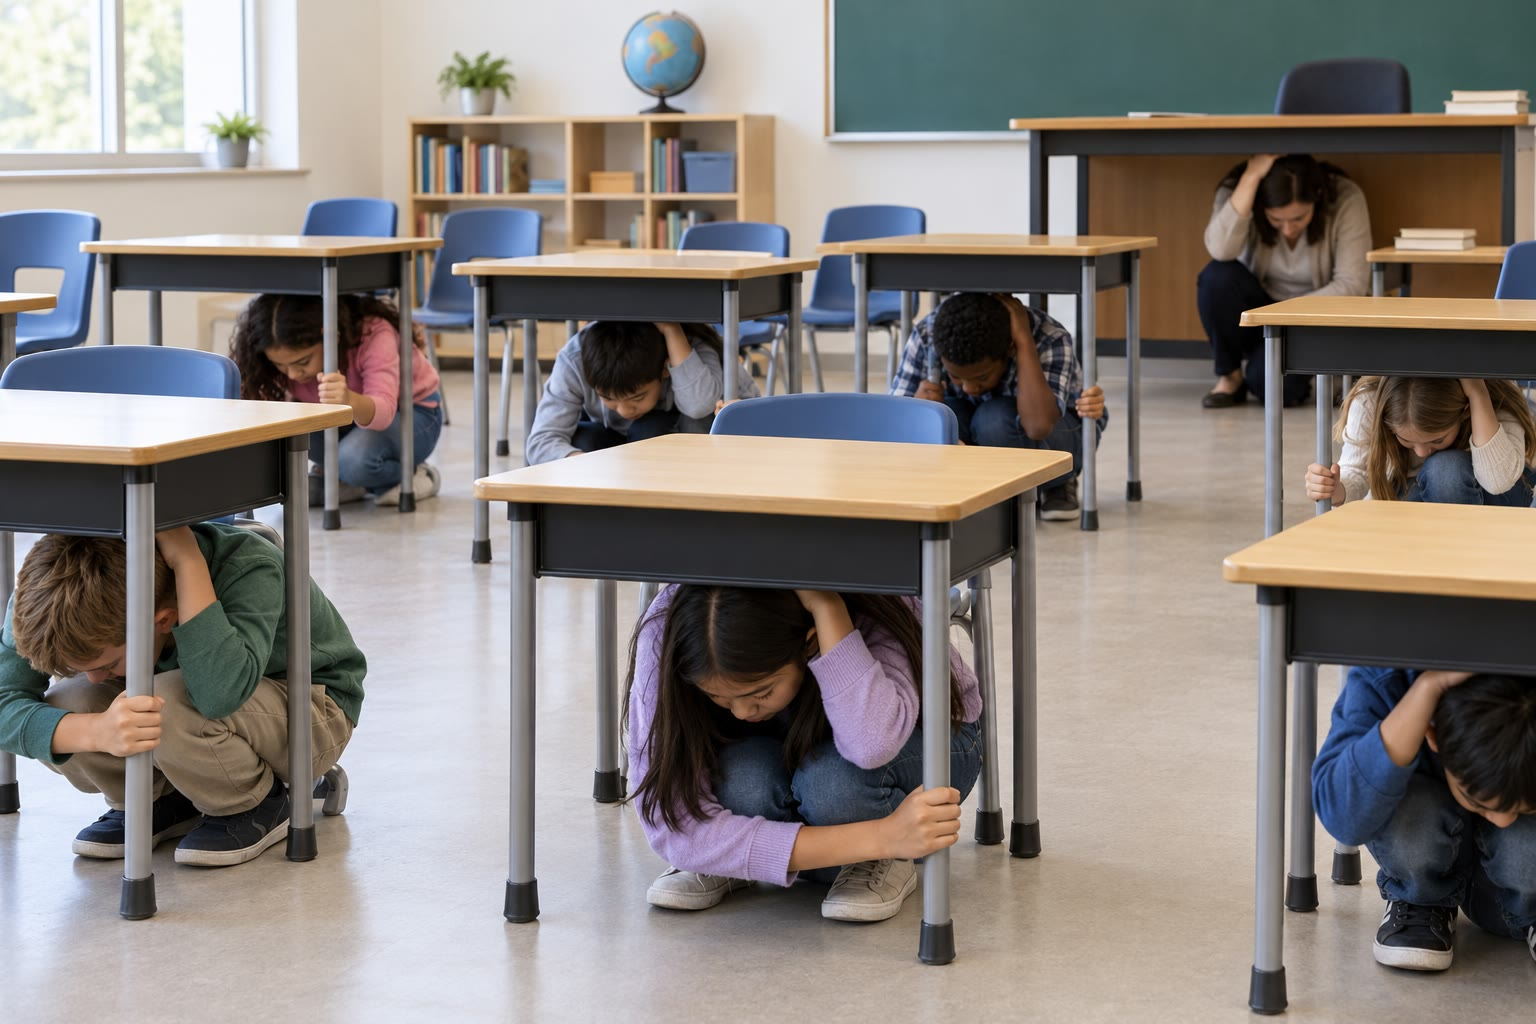
\includegraphics[width=0.55\linewidth]{images/book1/ai/g4-earthquake-drill.jpg}

{\small An \omterm{def:g4:volcanoes-earthquakes-first-look:earthquake}{earthquake} drill: the pupils practise ``drop, cover and hold
on'' under their tables.}
\end{omfigure}

\section{Exercises}

\begin{exercise}[$\star$]\label{exo:g4:volcanoes-earthquakes-first-look:1}
\omterm{def:g4:volcanoes-earthquakes-first-look:eruption}{Lava}, ash or gas? (a) a \omterm{def:g1:landscapes-around-us:water}{river} of glowing molten \omterm{def:g3:stones-pebbles-sand:rock}{rock} flowing down a slope;
(b) tiny pieces of \omterm{def:g3:stones-pebbles-sand:rock}{rock} blown into the sky, that fall back like grey \omterm{def:g4:clouds-rain-snow:precipitation}{snow};
(c) something invisible that escapes from the \omterm{def:g4:volcanoes-earthquakes-first-look:volcano}{volcano} with the ash.
\end{exercise}

\begin{exercise}[$\star$]\label{exo:g4:volcanoes-earthquakes-first-look:2}
What is an \omterm{def:g4:volcanoes-earthquakes-first-look:earthquake}{earthquake}? Does it last hours, or seconds?
\end{exercise}

\begin{exercise}[$\star$]\label{exo:g4:volcanoes-earthquakes-first-look:3}
Put the three steps in order: hold on; drop; cover.
\end{exercise}

\begin{exercise}[$\star$]\label{exo:g4:volcanoes-earthquakes-first-look:4}
On the \omterm{def:g2:drawing-to-map:map}{map} on page~\pageref{fig:g4:volcanoes-earthquakes-first-look:map}, around
which \omterm{def:g2:water-on-earth:ocean}{ocean} do most \omterm{def:g4:volcanoes-earthquakes-first-look:volcano}{volcanoes} lie?
\end{exercise}

\begin{exercise}[$\star$]\label{exo:g4:volcanoes-earthquakes-first-look:5}
True or false? (a) Most \omterm{def:g4:volcanoes-earthquakes-first-look:earthquake}{earthquakes} are too small to be felt. (b) \omterm{def:g4:volcanoes-earthquakes-first-look:eruption}{Lava}
stays liquid for ever. (c) When the ground shakes, the safest thing is to
run outside.
\end{exercise}

\begin{exercise}[$\star$]\label{exo:g4:volcanoes-earthquakes-first-look:6}
Look at the drawing of the \omterm{def:g4:volcanoes-earthquakes-first-look:volcano}{volcano} on page~\pageref{fig:g4:volcanoes-earthquakes-first-look:volcano}.
Where does the molten \omterm{def:g3:stones-pebbles-sand:rock}{rock} come from? Where does it come out?
\end{exercise}

\begin{exercise}[$\star\star$]\label{exo:g4:volcanoes-earthquakes-first-look:7}
On the \omterm{def:g2:drawing-to-map:map}{map}, find: (a) a country of the Americas with many \omterm{def:g4:volcanoes-earthquakes-first-look:volcano}{volcanoes} along
its whole length; (b) a group of islands in the middle of the Pacific
\omterm{def:g2:water-on-earth:ocean}{Ocean}, with \omterm{def:g4:volcanoes-earthquakes-first-look:volcano}{volcanoes}, that is not on the ring.
\end{exercise}

\begin{exercise}[$\star\star$]\label{exo:g4:volcanoes-earthquakes-first-look:8}
About 141 large \omterm{def:g4:volcanoes-earthquakes-first-look:earthquake}{earthquakes} happen in a year. About how many is that in a
month? (A year has 12 months; give a whole number.)
\end{exercise}

\begin{exercise}[$\star\star$]\label{exo:g4:volcanoes-earthquakes-first-look:9}
About 3 out of every 4 very large \omterm{def:g4:volcanoes-earthquakes-first-look:earthquake}{earthquakes} happen in the ring around the
Pacific. Out of 20 very large \omterm{def:g4:volcanoes-earthquakes-first-look:earthquake}{earthquakes}, about how many would you expect
in the ring? And outside it?
\end{exercise}

\begin{exercise}[$\star\star$]\label{exo:g4:volcanoes-earthquakes-first-look:10}
During an \omterm{def:g4:volcanoes-earthquakes-first-look:earthquake}{earthquake} drill, Leo runs to stand in the classroom doorway. What
should he have done instead, and why?
\end{exercise}

\begin{exercise}[$\star\star\star$]\label{exo:g4:volcanoes-earthquakes-first-look:11}
Of the 1\,214 \omterm{def:g4:volcanoes-earthquakes-first-look:volcano}{volcanoes} on the \omterm{def:g2:drawing-to-map:map}{map}, 837 are in the ring around the Pacific.
How many are outside it? Is ``about 2 out of 3'' a good way to describe the
share in the ring? (Hint: what is two thirds of 1\,200?)
\end{exercise}
